\begin{figure}
\tikzstyle{arrow} = [thick,->,>=stealth]
\tikzstyle{arrowd} = [thick,dashed,->,>=stealth]
\centering
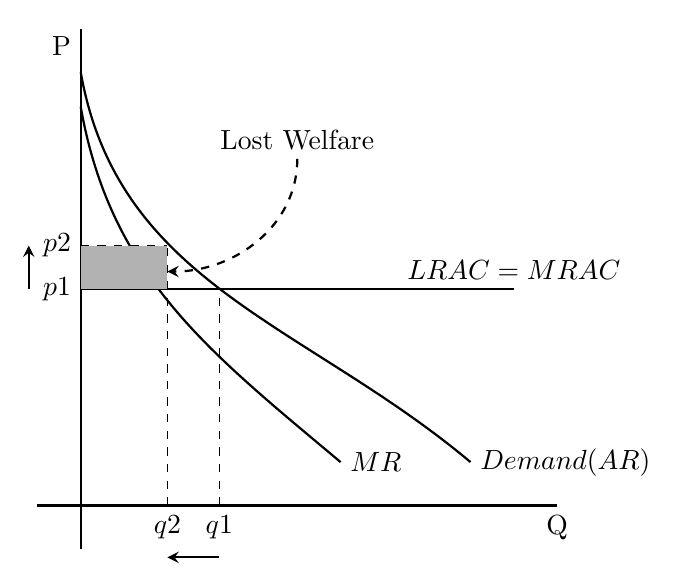
\begin{tikzpicture}[scale=1.1]

% Axis
\draw [thick] (-0.5,-0.0) --(5.5,0);
\draw [thick] (0,-0.5) -- (0,5.5);
\node [left] at (0,5.3) {P};
\node [below] at (5.5,0) {Q};

%Downward slopping line AR
\draw [thick] (0,5) to [out=280,in=140] (4.5,0.5);
\node [right] at (4.5,0.5) {$Demand (AR)$};

%Downward slopping line MR
\draw [thick] (0,4.6) to [out=280,in=140] (3,0.5);
\node [right] at (3,0.5) {$MR$};


% Upward Slopping S1
\draw [thick] (0,2.5) to (5,2.5);
\node [above] at (5,2.5) {$LRAC=MRAC$};

% dashed lines
\draw [dashed](1.6,0)--(1.6,2.5);
\draw [dashed](1,0)--(1,3);
\draw [dashed](0,3)--(1,3);

% Prices and Quantities
\node [left] at (0,3) {$p2$};
\node [left] at (0,2.5) {$p1$};
\node [below] at (1,0) {$q2$};
\node [below] at (1.6,0) {$q1$};

\draw [arrow](1.6,-0.6) -- (1,-0.6);
\draw [arrow](-0.6,2.5) -- (-0.6,3);

% lost welfare
\node [above] at (2.5,4) {Lost  Welfare};
\draw [arrowd](2.5,4) to [out=270,in=360](1,2.7);
\fill [black!30] (0,3) rectangle (1,2.5);

\end{tikzpicture}
  \caption{Figure showing welfare loss caused by monopoly abuse.}
  \label{fig:welfare_loss_monopoly}
\end{figure}